\documentclass[12pt, a4]{article}
\usepackage[english]{babel}
\usepackage[utf8x]{inputenc}
\usepackage{fullpage}
\usepackage{listings}
\usepackage{graphicx}
\usepackage{color}

%Syntax highlighting
\definecolor{blue-violet}{rgb}{0.54, 0.17, 0.89}
\definecolor{ao}{rgb}{0.0, 0.5, 0.0}
\definecolor{amaranth}{rgb}{0.9, 0.17, 0.31}
\definecolor{ballblue}{rgb}{0.13, 0.67, 0.8}
\definecolor{onyx}{rgb}{0.06, 0.06, 0.06}


\lstset{
  breaklines=true,                 % automatic line breaking only at whitespace
  captionpos=b,                    % sets the caption-position to bottom
  breakatwhitespace=false,
  keepspaces=true,
  numbers=left,
  numbersep=5pt,
  showspaces=false,
  showstringspaces=false,
  showtabs=false,
  tabsize=4,  
  backgroundcolor=\color{white},   % choose the background color
  commentstyle=\color{ao},    % comment style
  keywordstyle=\color{amaranth},    % keyword style
  stringstyle=\color{blue-violet},    % string literal style
  numberstyle=\tiny\color{ballblue},	   % number style
  basicstyle=\ttfamily\footnotesize\color{onyx} % size of fonts used for the code
}

%Document Header
\title{\textbf{Department of CSE\\SSN College of Engineering}}
\author{\textbf{Vishakan Subramanian - 18 5001 196 - Semester VII}}
\date{31 July 2021}

\begin{document}
\maketitle
\hrule
\section*{\center{UCS 1712 - Graphics And Multimedia Lab}}
\hrule
\bigskip

%Assignment Details
\subsection*{\center{\textbf{Exercise 2: Line Drawing Using Digital Differential Analyzer Algorithm}}}
\subsection*{\flushleft{Aim:}}
\begin{flushleft}
To plot points that make up the line with endpoints (x0, y0) and (xn, yn) using DDA line drawing algorithm.

\begin{itemize}
\item Case 1: +ve slope Left to Right line
\item Case 2: +ve slope Right to Left line
\item Case 3: -ve slope Left to Right line
\item Case 4: -ve slope Right to Left line
\end{itemize}
Each case has two subdivisions
(i) $|m| <= 1$ (ii) $|m| > 1$
\newline
\newline
Note that all four cases of line drawing must be given as test cases. 
\end{flushleft}

%Code
\newpage
\subsection*{\flushleft{Code: DDA:}}
\begin{flushleft}
\lstinputlisting[language = C]{DDA/main.cpp}
\end{flushleft}


%Output
\newpage
\subsection*{\flushleft{Output: DDA Case 1 - (0, 0) to (800, 600):}}
\begin{figure}[h]
\centering
\caption{Output: DDA, M $<=$ 1, Left to Right Line.}
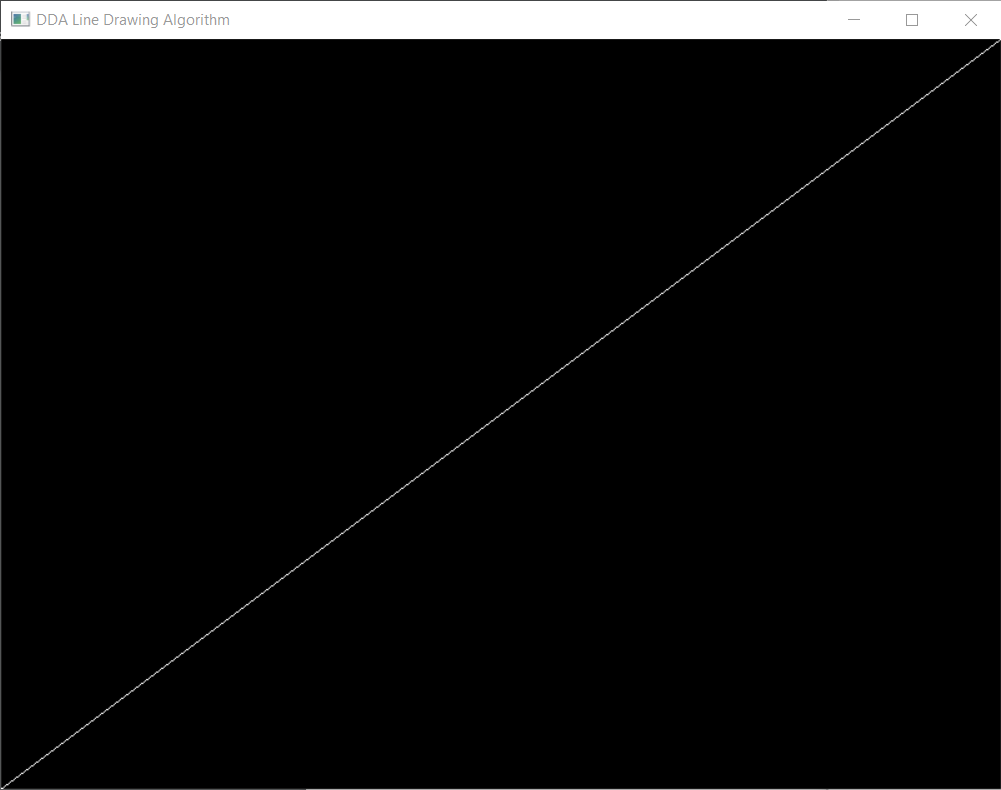
\includegraphics[height=11.25cm, width=15cm]{Outputs/1-DDA.png}
\end{figure}

%Output
\newpage
\subsection*{\flushleft{Output: DDA Case 2 - (800, 600) to (0, 0):}}
\begin{figure}[h]
\centering
\caption{Output: DDA, M $<=$ 1, Right to Left Line.}
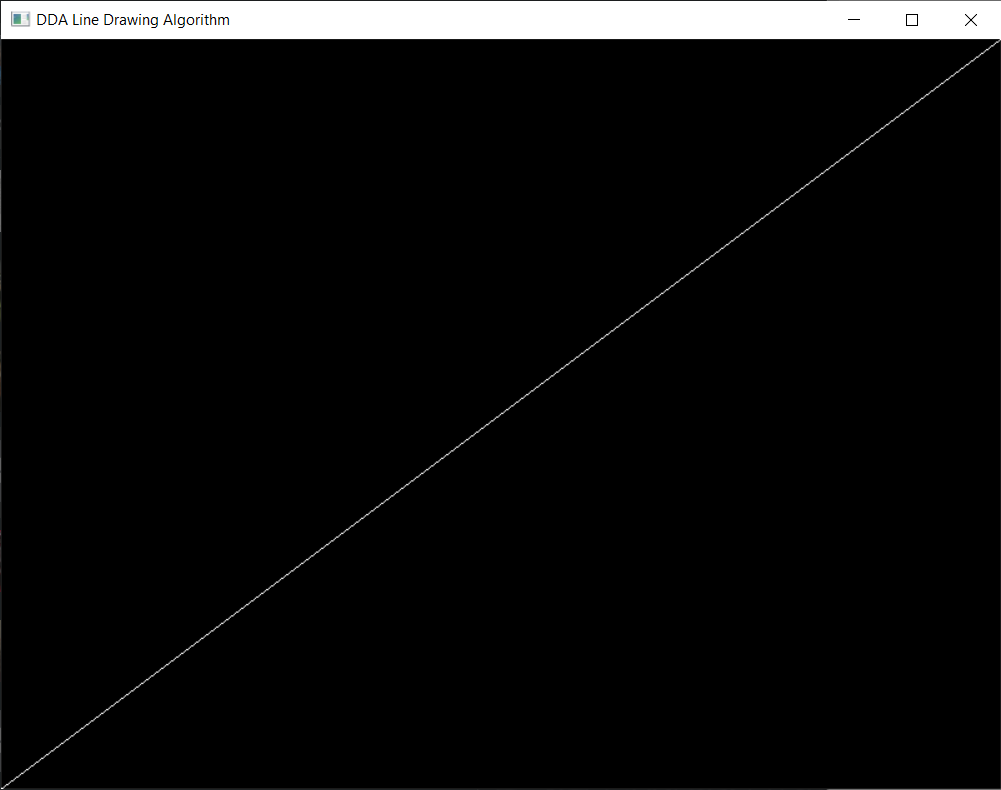
\includegraphics[height=11.25cm, width=15cm]{Outputs/2-DDA.png}
\end{figure}

%Output
\newpage
\subsection*{\flushleft{Output: DDA Case 3 - (200, 150) to (400, 500):}}
\begin{figure}[h]
\centering
\caption{Output: DDA, M $>$ 1, Left to Right Line.}
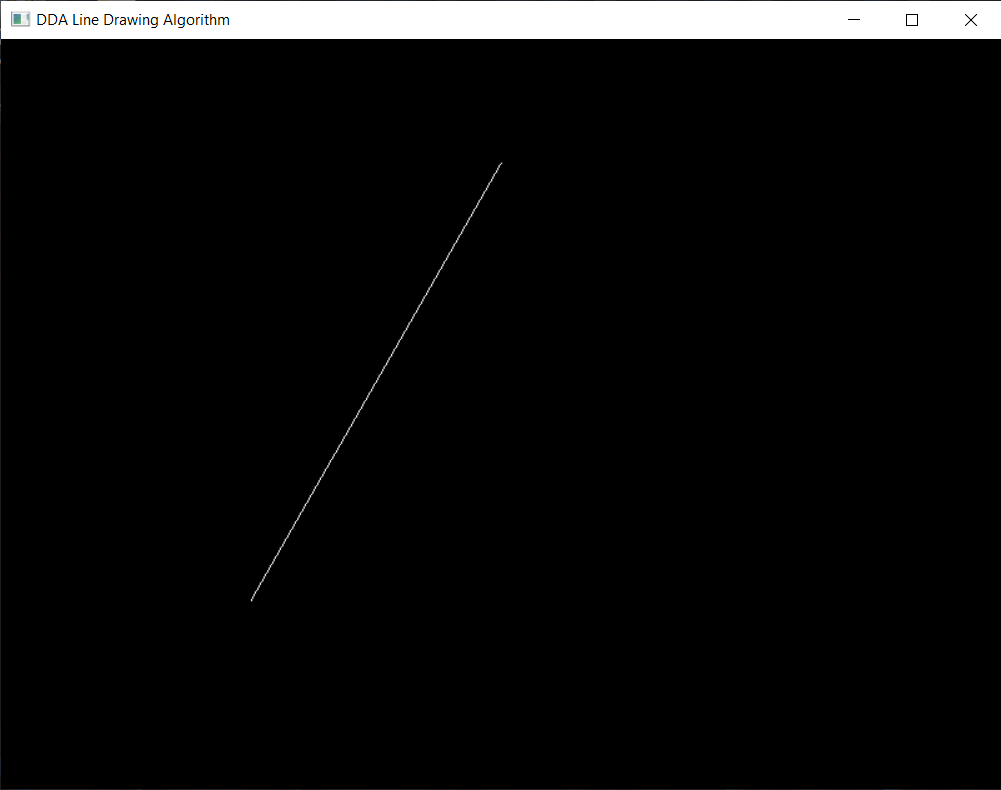
\includegraphics[height=11.25cm, width=15cm]{Outputs/3-DDA.png}
\end{figure}

%Output
\newpage
\subsection*{\flushleft{Output: DDA Case 4 - (400, 500) to (200, 150):}}
\begin{figure}[h]
\centering
\caption{Output: DDA, M $>$ 1, Right to Left Line.}
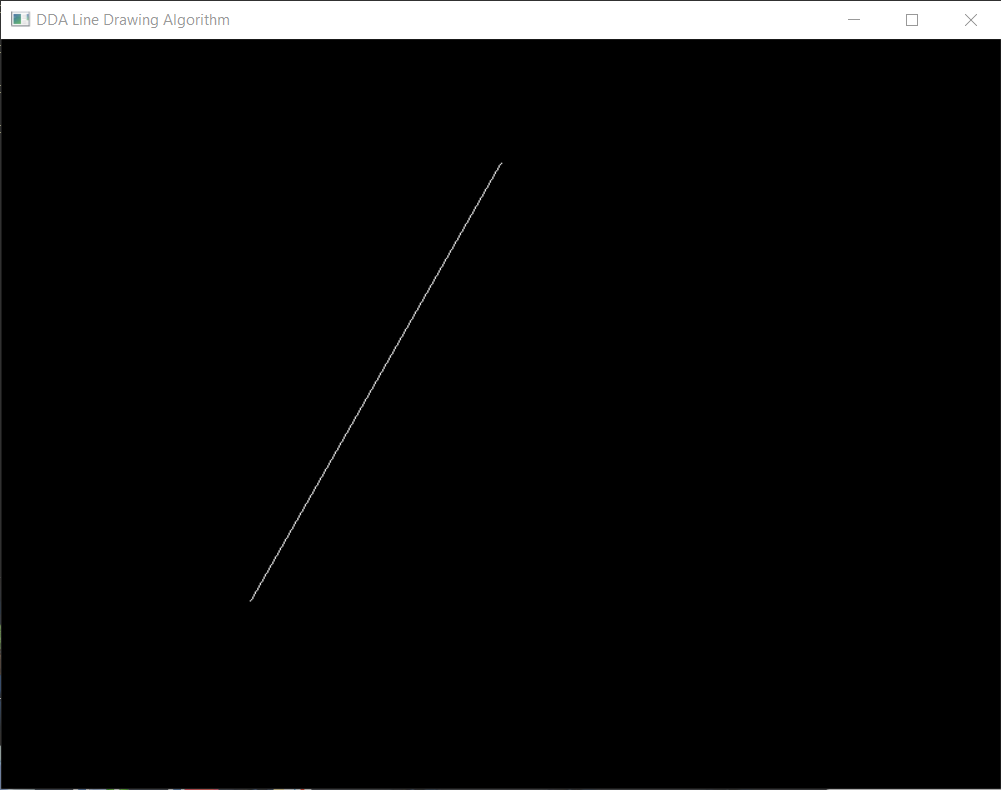
\includegraphics[height=11.25cm, width=15cm]{Outputs/4-DDA.png}
\end{figure}



%Learning Outcome
\newpage
\subsection*{\flushleft{Learning Outcome:}}
\begin{itemize}
\item I understood the \textbf{Digital Differential Analyzer Algorithm}'s working.
\item I implemented the DDA Algorithm using an OpenGL program.
\item I understood how points are plotted and how increments are calculated based on slope \& $\Delta x \; and \; \Delta y$ values in DDA Algorithm.
\item I understood that DDA Algorithm makes fine approximations and rounding off's which might be a pitfall when accurate diagrams are required.
\item I understood that DDA Algorithm is less efficient and less precise than the Bresenham's Line Algorithm.
\item I was able to output all different test cases appropriately to verify the correctness of my program to implement DDA Algorithm.

\end{itemize}


\end{document}